% !TEX root = ../thesis-example.tex
%
\chapter{Neutrino Masses from Combined Cosmological Probes and Oscillation Experiments Constraints}
\label{Chap:Neutrinos}

\cleanchapterquote{You can’t crush ideas by suppressing them. You can only crush them by ignoring them. By refusing to think, refusing to change.}{Ursula K. Le Guin}{(The Dispossessed)}

\vspace*{\fill}

In this chapter, I investigate the impact of prior models on the upper bound of the sum of neutrino masses, \NM{}. I use a combination of datasets: Large Scale Structure of galaxies, Cosmic Microwave Background, Type Ia SuperNovae, and Big Bang Nucleosynthesis. I analyse physically motivated models (or exact models), which respect oscillation experiment constraints from particle physics, and compare them to constraints using standard cosmological approximations. The former give a consistent upper bound of $\sum m_{\nu} \lesssim 0.26$ eV (95\% CI) and yields a strong competitive upper bound for the lightest neutrino mass species, $m_0^{\nu} < 0.086$ eV (95\% CI). This is one of the first ever constraints set to the mass of the lightest neutrinos in the literature. By contrast one of the cosmological approximations, which is somewhat inconsistent with oscillation experiments, yields an upper bound of $\sum m_{\nu} \lesssim 0.15$ eV (95\% CI), which differs substantially from the former upper bound. I, therefore, argue that cosmological neutrino mass and hierarchy determination should be pursued using physically motivated models, taking into account knowledge from oscillation experiments, since approximations might lead to incorrect and nonphysical bounds.

\textit{The work in this chapter was presented in \citet{2018LoureiroNeutrinos}.} 

\newpage
\section{Introduction}
Particle physics experiments in the late 1990s, such as Super-Kamiokande \citep{Kamiokande1998}, and recent experiments, such as SNO \citep{2002SNO}, KamLAND \citep{2005KamLAND}, and others \citep{2008MINOS,2012RENOExperiment,AbeNeutrino2014}, have established the existence of massive neutrinos, taking a first step beyond the Standard Model of Particle Physics. The missing solar neutrino problem, an apparent discrepancy between the observed and predicted number of $\nu_e$ originated by the Sun, was solved by understanding that such particles change between the three known leptonian flavours: $\nu_e, \, \nu_{\mu}$, and $\nu_{\tau}$ \citep{2016Capozzi}. As the solar neutrino detector was sensitive only to the electron neutrino, $\nu_e$, fewer particles were detected due to neutrinos changing their \textit{flavours}. This oscillation between neutrino flavours implies that these particles have non-vanishing mass eigen-states, denoted: $m_1$, $m_2$, and $m_3$. 
%\andrei{This is andrei's comments}

\qquad Recent global fits to data from several neutrino oscillations experiments obtained constraints for two different mass squared splittings \citep{2014Gonzalez-GarciaNeutrino}; from solar neutrino experiments,
\begin{equation}
\Delta m_{21}^2 \equiv m_2^2 - m_1^2 \approx 7.49^{+0.19}_{-0.17} \times 10^{-5} \text{eV}^2\, ,
\end{equation}  

and from atmospheric neutrinos, 
\begin{equation}
|\Delta m_{31}^2| \equiv |m^2_3 - m_1^2| \approx 2.484^{+0.045}_{-0.048} \times 10^{-3} \text{eV}^2
\end{equation}

both with 1-$\sigma$ error-bars. These measurements imply that at least two of the neutrino mass-eigenstates are non-zero and, given that the sign of $\Delta m_{31}^2$ is unknown, that two scenarios are possible, related to the ordering of the masses: $m_1 < m_2 \ll m_3$, known as the \textit{normal hierarchy} (NH), or $m_3 \ll m_1 < m_2$, the \textit{inverted hierarchy} (IH). Current neutrino experiments will not be able to break the degeneracy between these two hierarchies (or orderings) in the near future \citep{2014Blennow}. However, by considering the lightest neutrino mass eigenstate to be zero one can see that these experiments set a lower bound for the sum of neutrino masses,  $\sum m_{\nu} \equiv \sum_{i=1}^3 m_{\nu, i}$, as follows:  $\sum m_{\nu}^{NH} > 0.0585 \pm 0.00048$ eV or $\sum m_{\nu}^{IH} > 0.0986 \pm 0.00085$ eV \citep{2016Hannestad,2018UpdateNeutrinoMass,2018LongNeutrinoMassPior}.
%Recent global fits to neutrino oscillations experiments data from Ref. \citep{2014Gonzalez-GarciaNeutrino} obtained constraints for two different mass squared splittings: from solar neutrino experiments, $\Delta m_{21}^2 \equiv m_2^2 - m_1^2 \approx 7.49^{+0.19}_{-0.17} \times 10^{-5}$ eV$^2$; and from atmospheric neutrinos, $|\Delta m_{31}|^2 \equiv |m^2_3 - m_1^2| \approx 2.484^{+0.045}_{-0.048} \times 10^{-3}$ eV$^2$ (1-$\sigma$ error-bars). These measurements imply that at least two of the neutrino mass-eigenstates are non-zero and, given that the sign of $\Delta m_{31}^2$ is unknown, two scenarios occur related to the ordering of the masses: $m_1 < m_2 \ll m_3$, known as \textit{the normal hierarchy} (NH); or $m_3 \ll m_1 < m_2$, known as the \textit{inverted hierarchy} (IH). Current neutrino oscillation experiments cannot break the degeneracy between these two hierarchies (or orderings) in the next following years \citep{2014Blennow}. However, from these experiments, a lower bound can be set for the sum of neutrino masses,  $\sum m_{\nu} \equiv \sum_{i=1}^3 m_{\nu, i}= m_1 + m_2 + m_3$, considering the lightest neutrino mass-eigenstate to be zero: $\sum m_{\nu}^{NH} > 0.0585 \pm 0.00048$ eV or $\sum m_{\nu}^{IH} > 0.0986 \pm 0.00085$ eV \citep{2016JCAP...11..035H,2018UpdateNeutrinoMass}.

\qquad From a different perspective, cosmological surveys have the potential to probe the sum of neutrino masses \citep{2007FBA,Thomas2010Neutr}, and also to constrain the neutrino mass hierarchy \citep{2003HannestadNeutrino,2016Hannestad}. The large scale structure of galaxies in the Universe is sensitive to the sum of neutrino masses and the number of massive neutrino species, $N_{\nu}$, since the cosmic energy density ratio for massive neutrinos in a $\Lambda$CDM model is

\begin{equation}
\label{Eq:NeutrinoOmega}
    \Omega_{\nu} = \sum_i^{N_{\nu}}\left[\left(\frac{G}{\pi^2H_0^2}\right)\int d^3p_i \frac{\sqrt[]{p_i^2 + m_{\nu,i}^2}}{(e^{p_i/T_{\nu,i}} + 1)} \right].
\end{equation} 

\noindent For the case of degenerate masses and after neutrinos start behaving non-relativistically, this can be approximated by \citep{Thomas2010Neutr}
\begin{equation}
    \Omega_{\nu} \approx \frac{\sum m_{\nu}}{(92.5\, h^2\text{eV})}\, .
\end{equation}
This approximation is at the core of the approach taken by most cosmological analyses when probing the related neutrino parameters; this leads to  95\% CI upper bounds on \NM{} as low as $< 0.12$ eV from Ly-$\alpha$ measurements \citep{2015LyAlpha-Deg} and also from the latest Planck Collaboration results \citep{2018PlanckCosmology}. A complete review of neutrino mass ordering in cosmology and particle physics can be found in \cite{2012Julien-Deg} and \cite{2018MassOrdering}.

\qquad In this chapter, I investigate the sensitivity of the angular power spectra of galaxies to massive neutrino parameters by analysing the impact such parameters have in the $C_{\ell}$s. Next, I present different ways to model the sum of neutrino masses in cosmology in order to analyse the impact of different classes of neutrino mass modelling strategies on cosmological parameters and neutrino constraints. This test is performed with the latest cosmological data, namely a tomographic analysis in harmonic space applied to the largest spectroscopic galaxy sample to date, the BOSS DR12 \citep[][-- also presented in Chapter \ref{Chap:BOSS}]{2018LoureiroBOSS}, combined with Planck cosmic microwave background (CMB) temperature, polarisation, and lensing \citep{PlanckCosmology2016}, Pantheon supernovae compilation data \citep{2018Pantheon}, BBN measurements of the deuterium-hydrogen fraction \citep{2018BBN-Measurements}, and, in some of the models, the latest neutrino mass squared splitting constraints from particle physics \citep{2014Gonzalez-GarciaNeutrino}.


\section{Neutrino Mass Effects in Harmonic Space}
\begin{figure}
\begin{center}
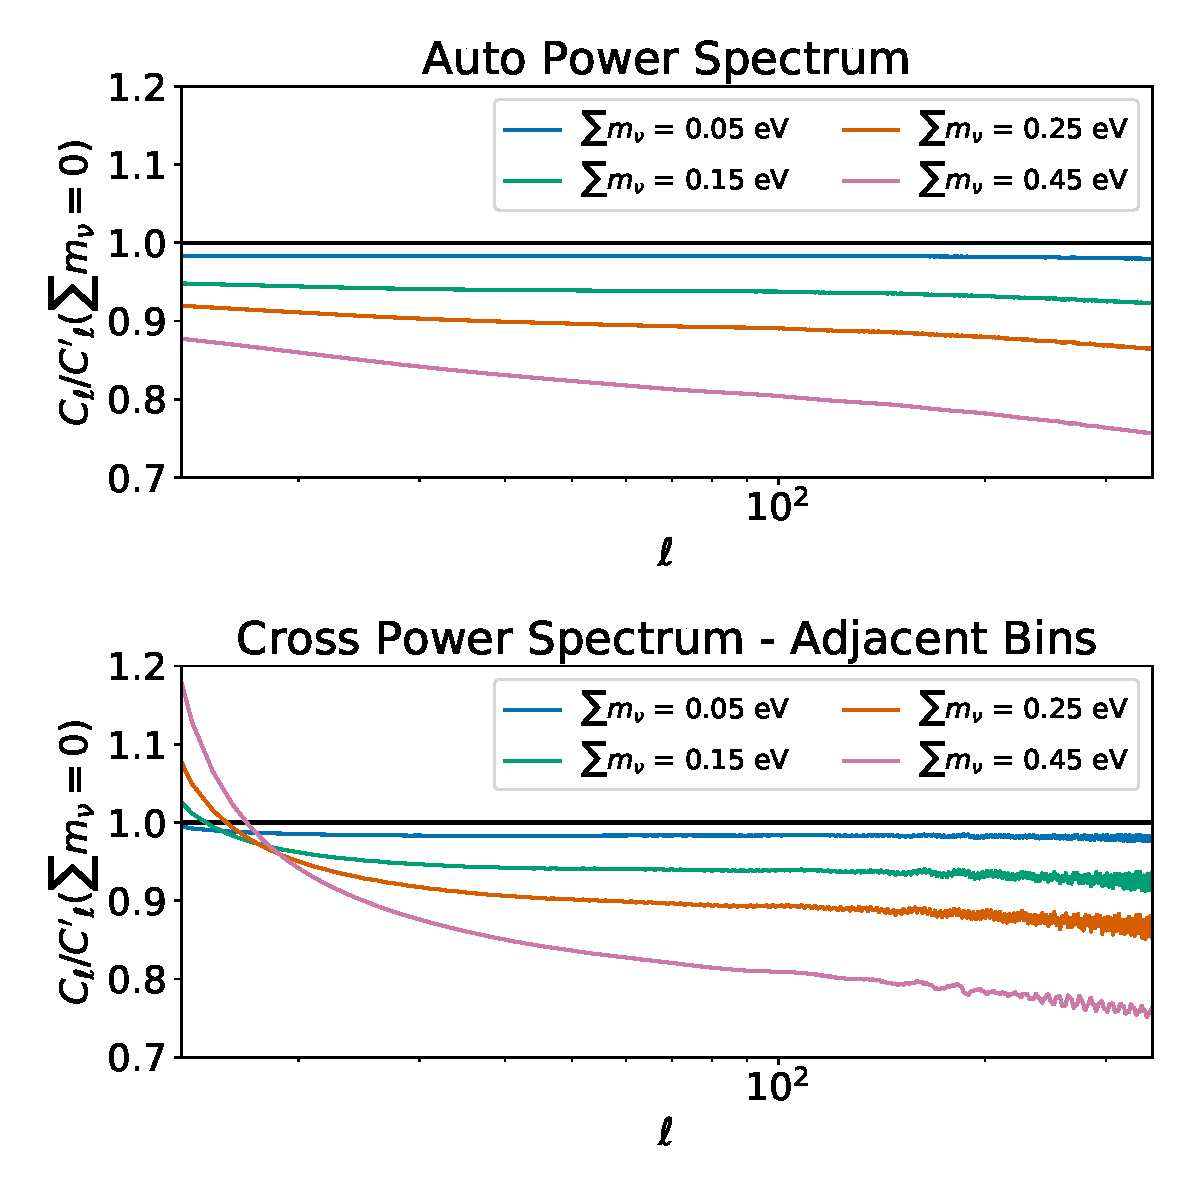
\includegraphics[scale=0.50]{Neutrino-FIGS/Neutrinos_SumMnu.pdf}
\caption[Impact of the sum of neutrino masses in the angular power spectra of galaxies.]{Impact of the sum of neutrino masses in the angular power spectra of BOSS galaxies shown as the ratio between $C_{\ell}$s calculated with different values of \NM{} over a case with no massive neutrinos, i.e. $\sum m_{\nu} = 0$ eV. \textit{(Top)} shows the ratio for the auto angular power spectra of a BOSS tomographic bin centred in $\bar{z} = 0.275$. \textit{(Bottom)} shows the ratio for the cross power spectrum between two BOSS bins, one centred in $\bar{z} = 0.275$ and its adjacent bin, $\bar{z} = 0.325$. Oscillations on the high-$\ell$ end of the spectrum are due to some numerical instabilities which do not affect the cosmological analysis due to band-width binning.}
\label{fig:neutrinoCompareSumM}
\end{center}
\end{figure}
Many works in the literature investigate the impact of massive neutrinos in the 3D power spectra or in the correlation function of galaxies \citep{2007FBA,2012Julien-Deg,Bird2012}. In a review \cite{2006NeutrinoReview}, it is shown how that for the 3D power spectrum of galaxies massive neutrinos suppress power after certain scales, $k \sim 5\times 10^{-3}$ h/Mpc; with a similar effect rising from the effective number of relativistic species, $N_{\text{eff}}$. The impact of massive neutrinos in the angular power spectra of galaxies is still to be explored as projection effects are so that it becomes unclear that the effect will be similar as that of the 3D power spectrum.

\qquad In this section, I make use of the \textit{Unified Cosmological Library for $C_{\ell}$s}, or \uclcl (Cuceu et al, \textit{in prep} -- benchmarked in Appendix \ref{Apx:Code_Comparison}), to generate theoretical predictions using a Planck-like fiducial cosmology\footnote{The fiducial $\Lambda$CDM cosmology used is $h=0.6725$, $\Omega_b = 0.0492$, $\Omega_{cdm} = 0.265$, $\ln 10^{10}A_s = 3.093$, $n_s = 0.965$, $\tau_r = 0.079$.} in order to investigate the impact of neutrino related parameters in the angular power spectra of galaxies. The objective of this study is to understand how sensitive the BOSS $C_{\ell}$s, presented in Chapter \ref{Chap:BOSS}, are to neutrino parameters. Therefore, I used the BOSS redshift distribution (as presented in Figure \ref{fig:NZ_BOSS}) and the same binning scheme as presented in Table \ref{Tb:Shells} to generate the theoretical $C_{\ell}$s; the bias and other nuisance parameters were kept to unity in order to simplify the analysis. For simplicity, figures displayed in this section show only an example of an auto power spectrum for a bin centred in $\bar{z} = 0.275$ and the cross power spectrum between this first bin and an adjacent one with $\bar{z} = 0.325$ -- both with $\Delta z = 0.05$.

\qquad There are three main parameters that will be considered in this section: the sum of neutrino masses, \NM{}, the effective number of relativistic species, $N_{\text{eff}}$, and the actual number of massive neutrinos, $N_{\nu}$.

\subsubsection{Impact of \NM{} in the galaxy angular power spectrum:}
In order to understand the impact of the sum of neutrino masses in the angular power spectra of galaxies, I kept the baryonic matter content of the Universe ($\Omega_b$) fixed as well as the curvature flat, i. e. $\Omega_{k} = 0$, meaning that $\sum_i \Omega_i = 1$. This implies that when varying the neutrino energy density via changing \NM{} (see Equation \ref{Eq:NeutrinoOmega}), $\Omega_{cdm}$ is not kept constant. Theoretical predictions were calculated for angular auto- and cross-power spectra between all BOSS redshift tomographic bins. Figure \ref{fig:neutrinoCompareSumM} shows an example of the ratio between different values of \NM{} against a case with no massive neutrinos for one auto- and one cross-power spectrum.

\qquad Differently from the usual 3D power spectrum analysis, it is clear from Figure \ref{fig:neutrinoCompareSumM} that massive neutrinos affect all scales (multipoles). This can only be explained by the fact that when performing a tomographic analysis, the radial scales get projected. The projection mixes the neutrino information (contained mostly in smaller scales for the 3D case) in a way that is now present in all multipoles. However, one must be careful when probing this parameter using $C_{\ell}$s from galaxy clustering. The more massive the total sum of neutrinos are, the more suppression of power occurs in all scales. From a different perspective, shot-noise also affects in the angular power spectra in all scales; however, the higher the shot-noise, the more increase of power in all scales is found. In Section \ref{Sec:nCDM}, it is pointed out how non-Poissonian (or extra) shot-noise, if not modelled correctly, could mimic low neutrino masses; Figure \ref{fig:neutrinoCompareSumM} confirms this statement. It is of fundamental importance to deal correctly with this effect. This becomes crucially important for spectroscopic galaxy surveys with very fine tomographic bins due to their small density of galaxies in each bin.

\subsubsection{Impact of $N_{\text{eff}}$ in the galaxy angular power spectrum:}
\begin{figure}
\begin{center}
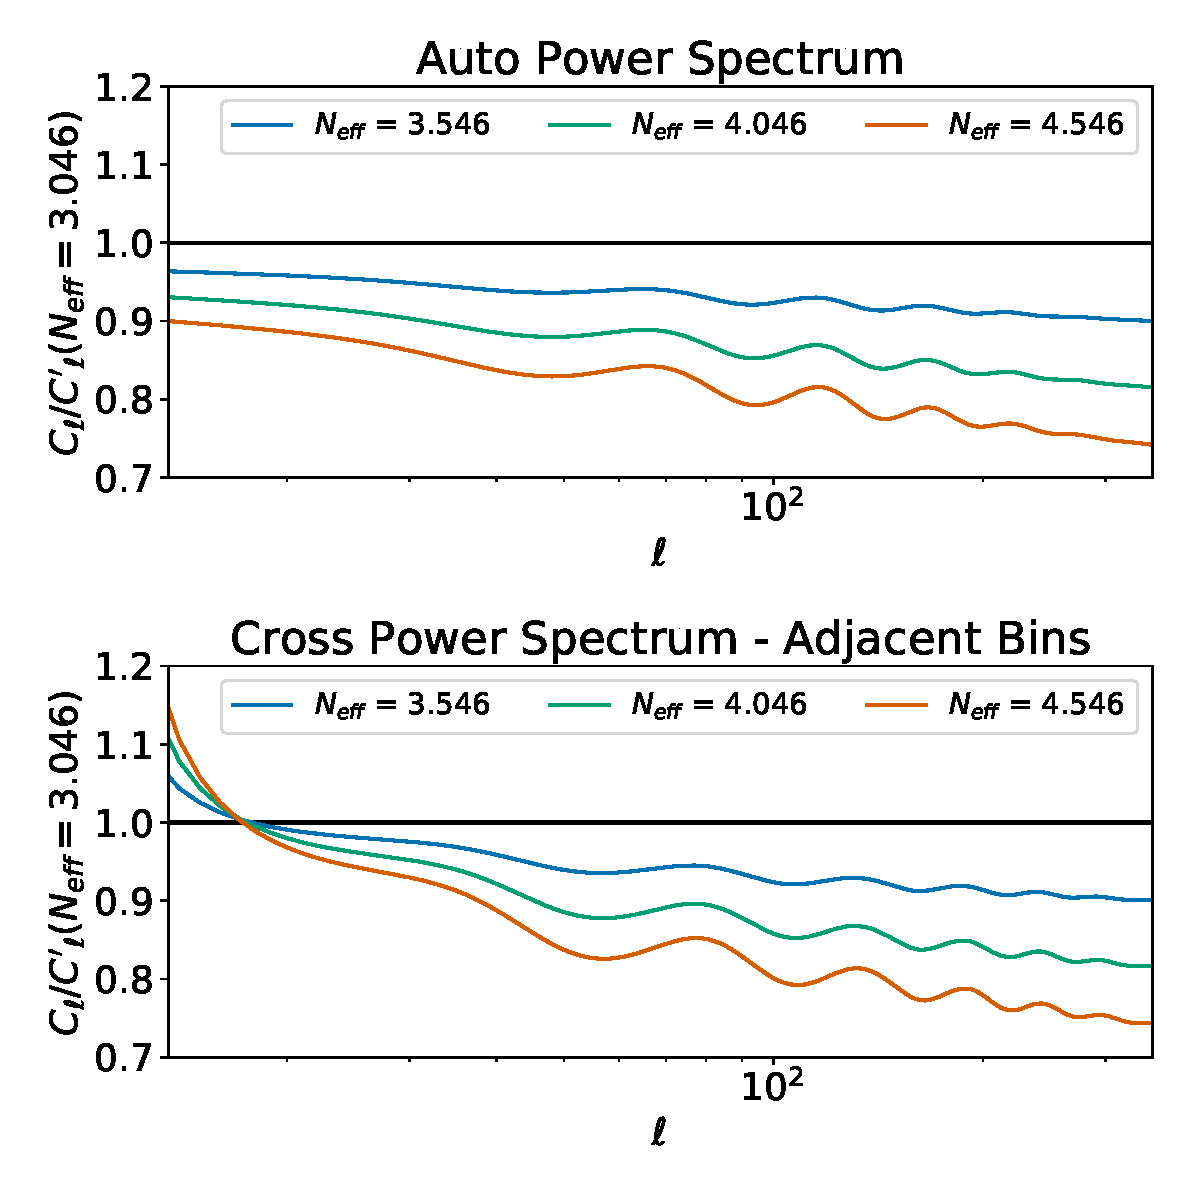
\includegraphics[scale=0.50]{Neutrino-FIGS/Neutrinos_Neff.pdf}
\caption[Impact of the effective number of relativistic species in the angular power spectra of galaxies.]{Ratio between $C_{\ell}$s with different values of $N_{\text{eff}}$ and $C_{\ell}$s containing $N_{\text{eff}} = 3.046$, the assumed fiducial value for $\Lambda$CDM. \textit{(Top)} Shows, as an example, the ratio between $C_{\ell}$ predictions for auto power spectrum of a BOSS tomographic bin with $\bar{z} = 0.275$. (Bottom) Same but for the cross power spectrum between adjacent bins centred in $\bar{z} = 0.275$ and $\bar{z} = 0.325$.}
\label{fig:neutrinoCompareNeff}
\end{center}
\end{figure}

The effective number of relativistic species is considered to be $N_{\text{eff}}\approx 3.046$. The reason this number not an integer is because it is also related to the temperature at which each massive neutrino species decouple from the other species and after the photon re-heating phase. Since not all neutrino species decouple at the same time, some species are still in thermal equilibrium with photons. As these photons get re-heated, some neutrinos will feel this effect, leading to a small excess of energy for this species. This can be dealt with by either probing each neutrino temperature separately with $N_{\text{eff}}=N_{\nu}$ or by considering $N_{\text{eff}}$ to be non-integer. The latter approach tends to be more efficient as it needs a much smaller parameter space.

\qquad From Figure \ref{fig:neutrinoCompareNeff}, one can see that, similarly to \NM, $N_{\text{eff}}$ affects all scales in the auto power spectrum of galaxies. However, the cross power spectrum demonstrates a different behaviour: for higher $N_{\text{eff}}$, higher is the increase of power for large scales while demonstrating a stronger suppression of power for small scales. A point of complete degeneracy can also be identified for small-$\ell$s. This different behaviour between angular auto- and cross-power spectra helps breaking some degeneracies when inferring cosmological parameters from this observational probe. If probing just the auto power spectra, the effect of $N_{\text{eff}}$ is similar to that of \NM{} and the shot-noise.

\subsubsection{Impact of $N_{\nu}$ in the galaxy angular power spectrum:}
\begin{figure}
\begin{center}
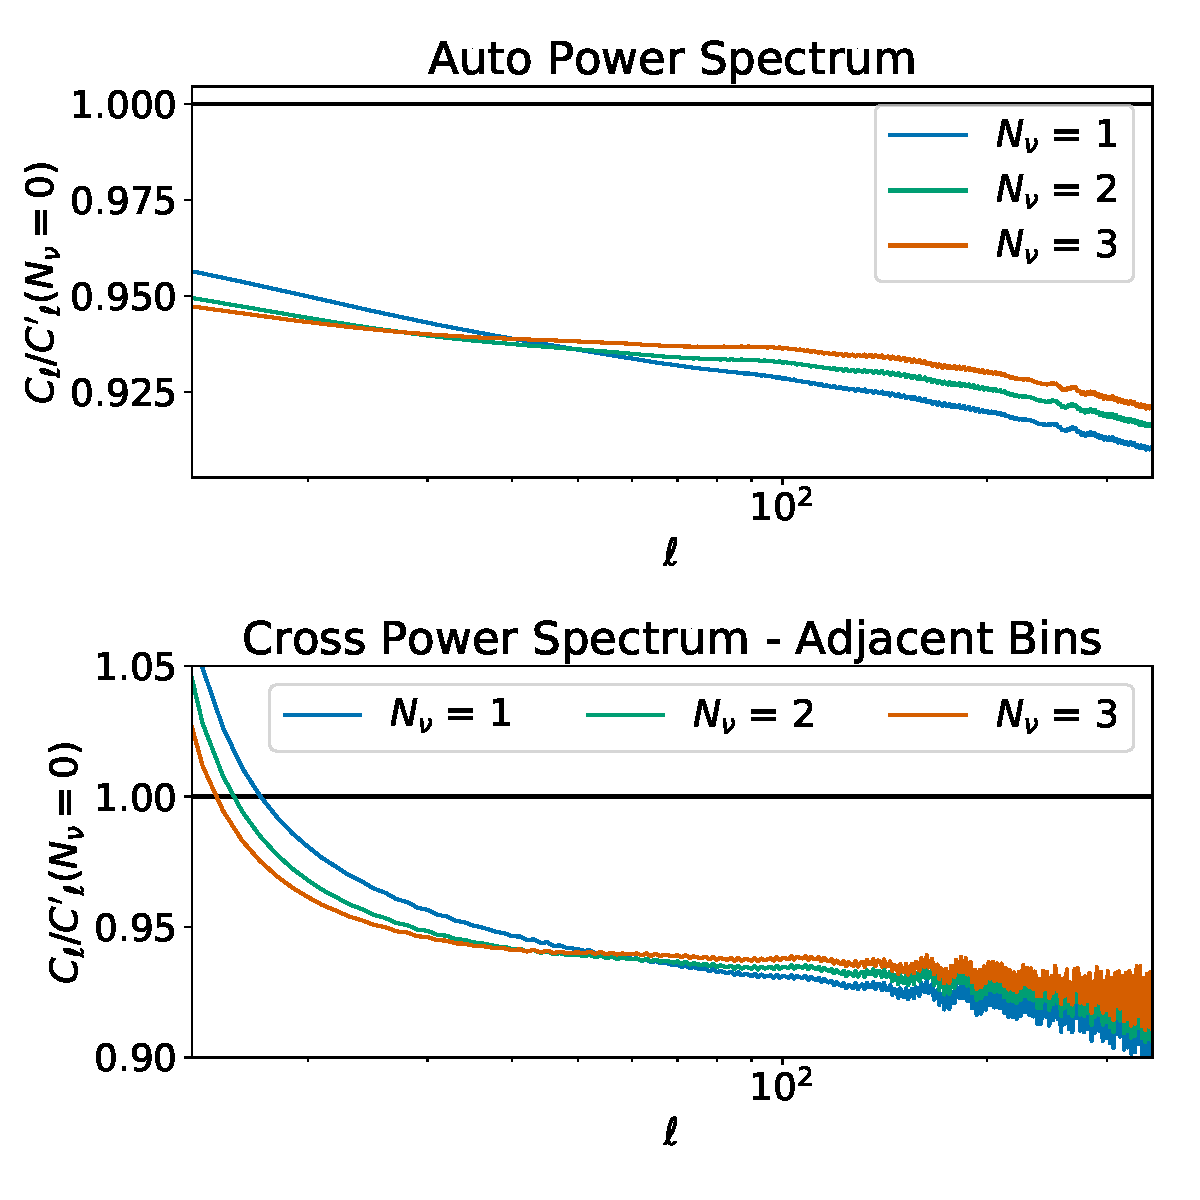
\includegraphics[scale=0.50]{Neutrino-FIGS/Neutrinos_Nnu.pdf}
\caption[Impact of the number massive neutrinos in the angular power spectra of galaxies.]{Ratio between $C_{\ell}$s with 1, 2 or 3 massive neutrinos against a case with no massive neutrino species. (Top) Ratio between the auto angular power spectra for different number of massive neutrinos for a redshift tomographic bin centred at $\bar{z} = 0.275$. (Bottom) Same ratio, now for the cross angular power spectra between adjacent bins centred at $\bar{z} = 0.275$ and $\bar{z} = 0.325$. Oscillations on the high-$\ell$ end of the spectrum are due to some numerical instabilities which are avoided using band-width binning in the cosmological analysis.}
\label{fig:neutrinoCompareNnu}
\end{center}
\end{figure}

From the three parameters related to neutrino properties analysed in this section, the number of massive neutrino species is the least sensitive of all when using clustering $C_{\ell}$s as a probe. Figure \ref{fig:neutrinoCompareNnu} shows that, although there is a significant difference between no massive neutrinos and $N_{\nu} > 0$, the difference between 1, 2 or 3 massive species is such that the current data considered in this work, the BOSS LSS sample, are not capable to distinguish between these scenarios when varying only this parameter. Even though the other parameters demonstrated a significant impact in the BOSS $C_{\ell}$s, the number of massive neutrino species is indistinguishable withing the estimated error-bars. This indicates the necessity of extra cosmological information from the CMB, SNe Ia, and BBN in order to probe all the considered neutrino mass properties.

\section{Neutrino Mass Models}

In this section, I describe the different neutrino models considered. These prior models are subdivided into two categories: exact models and cosmological approximations. The exact models incorporate particle physics constraints from neutrino oscillation experiments via modelling \NM{}, using a parametrisation based on the smallest neutrino mass, $m_0^{\nu}$ \citep{2012Hannestad,2016Hannestad,2018HeavensNeutrino}. For the normal hierarchy, one has:
\begin{align}
    \sum m_{\nu}^{NH} =\,  m^{\nu}_{0} & + \sqrt[]{\Delta m_{21}^2 + (m^{\nu}_{0})^2} + \sqrt[]{|\Delta m_{31}^2| + (m^{\nu}_{0})^2}
\end{align}
\noindent while in the inverted hierarchy: 
\begin{align}
    \sum m_{\nu}^{IH} =\,  m_0^{\nu} & + \sqrt[]{|\Delta m_{31}^2| + (m_0^{\nu})^2} + \sqrt[]{ |\Delta m_{31}^2| + \Delta m_{21}^2 + (m_0^{\nu})^2}.
\end{align} 
In what follows these will be referred to as the $m_0^{\nu}$-parametrisation. 

\qquad More explicitly, I consider four different exact models. \textit{Model 1} samples a binary switch parameter, $\mathcal{H}$, allowing the analysis to change between the two hierarchies with same prior volume, while also sampling the particle physics constraints for the mass splittings, $\Delta m_{21}^2$ and $|\Delta m_{31}^2|$, from Gaussian priors incorporating the errors in these measurements. \textit{Model 2} is similar to Model 1 but fixes the particle physics constraints to their central values: $\Delta m_{21}^2 = 7.49\times 10^{-5}$ eV$^2$ and $|\Delta m_{31}^2| = 2.484\times 10^{-3}$ eV$^2$. \textit{Model 3} (resp. \textit{Model 4}) fixes the mass splittings to their central values while also fixing the hierarchy to be normal (resp. inverted).

\qquad The second class of models, the cosmological approximations, are related to degenerated scenarios in which $\sum m_{\nu} = N_{\nu}\times m_{\text{eff}}$, where $m_{\text{eff}}$ is an effective mass, equal for each massive neutrino species. For each of these models, $N_{\nu}$ is fixed to a specific value and \NM{} is sampled. \textit{Model 5} is a NH approximation with $N_{\nu} = 1$, i.e., I approximate the two lower mass neutrino species to $m_1 = m_2 = 0$ \citep[][ -- also used in Chapter \ref{Chap:BOSS}]{2003HannestadNeutrino,2014Battye-Deg-1Mass,2016Giusarma-Deg-InvApp-NormAppr,PlanckCosmology2016,2018LoureiroBOSS}. Next, in a similar way, \textit{Model 6} is an IH approximation, where the lightest neutrino species is considered to be massless, which implies that $N_{\nu} = 2$ \citep{2016Giusarma-Deg-InvApp-NormAppr}. The last model in this class, \textit{Model 7}, is the most commonly used in standard cosmological analysis: the degenerate neutrino mass spectrum case, where $N_{\nu} = 3$ and $\sum m_{\nu} = 3m_{\text{eff}}$ \citep{2012Julien-Deg,2013Giusarma-Deg,2014Battye-Deg-1Mass,2015LyAlpha-Deg,2016Cuesta-Deg,2016BOSSCosmology,2016Giusarma-Deg-InvApp-NormAppr,2017Achidiacono-Deg,2017Cuchout-DegCase,2018PlanckCosmology,2017Vagnozzi-3deg,2018UpdateNeutrinoMass}. 

\qquad I also compared these seven models to cases where the \NM{} parameter is fixed to the most common values found in the literature for $\Lambda$CDM analysis \citep{2017arXiv170801530D,2017MNRAS.465.1454H,2018PlanckCosmology,2016BOSSCosmology}. \textit{Model 8} assumes no massive neutrinos; while \textit{Model 9} fixes it to the minimum possible value for the NH, $\sum m_{\nu} = 0.06$ eV, and sets $N_{\nu} = 3$ (as in the $\Lambda$CDM approach taken by the Planck Collaboration \citep{PlanckCosmology2016,PlanckResults2015}).

\qquad A summary of each model, together with the relevant neutrino mass parameters sampled %and the upper bounds for \NM{} and $m_{0}^{\nu}$ at 95\% credible interval (CI), 
can be found in Table \ref{Tb:Models1}.

\begin{table*}
  \centering
  \caption{A summary of the neutrino mass models considered in this chapter and the neutrino-related parameters sampled in each case.}
  \label{Tb:Models1}
  \begin{tabular}{cp{80mm}|c}
    \hline
    \hline
    Model & Description & $\nu$-Parameters\\[0.1cm]
    \hline
    \hline
    
     1 & Both hierarchies, $m_0^{\nu}$-parametrisation, sampling $|\Delta m_{31}^2|$ and $\Delta m_{21}^2$ from Gaussian priors. &  $m_0^{\nu}$, $\mathcal{H}$, $|\Delta m_{31}^2|$, $\Delta m_{21}^2$  \\
     
     2 & Both hierarchies,  $m_0^{\nu}$-parametrisation with $|\Delta m_{31}^2|$ and $\Delta m_{21}^2$ fixed to their central value. &  $m_0^{\nu}$, $\mathcal{H}$ \\
     
     3 & Normal Hierarchy,  $m_0^{\nu}$-parametrisation, fixed mass splittings. &  $m_0^{\nu}$ \\
     
     4 & Inverted Hierarchy,  $m_0^{\nu}$-parametrisation, fixed mass splittings. &  $m_0^{\nu}$ \\
     
     \hline
     5 & Normal Hierarchy approximation, $N_{\nu}=1$.  &  $\sum m_{\nu}$ \\
     
     6 & Inverted Hierarchy approximation, $N_{\nu}=2$. &  $\sum m_{\nu}$ \\
     
     7 & Degenerated masses approximation, $N_{\nu}=3$. & $\sum m_{\nu}$ \\
     \hline
     8 & No massive neutrinos, i.e., $N_{\nu}=0$ &   -- \\
     9 & Fixed to Normal Hierarchy's lower bound, $\sum m_{\nu} = 0.06$ eV &  -- \\
     \hline
     \hline 
  \end{tabular}
\end{table*}

\section{Assumptions}
\begin{table}
  \centering
  \caption{Ranges of priors used in all Bayesian analysis. All parameters sampled from flat priors with the exception of $\Delta m_{21}^2$ and $|\Delta m_{31}^2|$ which were sampled from Gaussians, $\mathcal{G}(\mu,\sigma)$. Parameters are divided into three groups: cosmological, neutrinos, and nuisance. Note that different models have different combinations of parameters.}
  \label{Tb:PriorsNeutrinos}
  \begin{tabular}{cc}
    \hline
    \hline
    Parameter & Prior Range \\
    \hline
    \hline
     $\Omega_b$ & $1 \times 10^{-3}, \, 0.3$    \\
     $\Omega_{cdm}$ & $0.0, \, 0.8$    \\[0.1cm]
     $\ln 10^{10} A_s$ & $2.0, \, 4.0$    \\
     $n_s$ & $0.87, \, 1.07$    \\
     $h$ & $0.55,\, 0.91$ \\
     $\tau^{Planck}_{reio}$  & $0.0,\, 0.8$ \\
     \hline
     $\sum m_{\nu}$ & $0.0,\, 1.0$ eV\\[0.1cm]
     $m^{\nu}_0$ & $1\times 10^{-4},\, 0.3$ eV \\
     $N_{\text{ur}}$ & $-N_{\nu},(6-N_{\nu})$ \\
     $\Delta m_{21}^2$ & $\mathcal{G}(\mu = 7.49, \sigma = 0.19)\times 10^{-5} eV^2$\\
     $|\Delta m_{31}^2|$ & $\mathcal{G}(\mu = 2.484, \sigma = 0.048)\times 10^{-3} eV^2$ \\
     \hline
     $b(z)$  & $1.1,\, 3.3$ \\
     $\sigma_s(z)$ & $1 \times 10^{-6},\, 9 \times 10^{-3}$ \\
     $\mathcal{N}_{11}$ & $0.0, \, 8\times 10^{-5}$ \\
     $\mathcal{N}_{12}$ & $0.0, \, 4\times 10^{-4}$ \\
     $y_{cal}^{Planck}$ & $0.99, \, 1.01$ \\
     $M_B^{SNe}$ & $-20.0,\, -18.5$\\
     \hline
     \hline
  \end{tabular}
\end{table}
Since the most recent analysis from the Planck Collaboration demonstrates that the Universe is flat to within 0.2\% precision, in this analysis I assume a flat $\Lambda$CDM scenario with massive neutrinos. The equation-of-state of dark energy is fixed to the cosmological constant case, $w=-1$. I also assume the possibility of extra effective ultra-relativistic particles, which are probed via the $N_{ur}$ parameter -- this parameter is degenerate with the decoupling of massive neutrinos at different temperatures and for simplicity I assume the same decoupling temperature. As the galaxy clustering information comes from BOSS DR12 angular power spectra, no fiducial cosmology was assumed for this sample (as explained in \cite{2018LoureiroBOSS} -- as well as in Chapter \ref{Chap:BOSS}). Priors for the standard $\Lambda$CDM parameters and nuisance parameters are described in Table \ref{Tb:PriorsNeutrinos} -- all priors were chosen to be flat, with the exception of the data-driven priors from neutrino oscillation experiments, $\Delta m_{21}^2$ and $|\Delta m_{31}^2|$, which are Gaussian priors. The priors were chosen based on previous works in the literature \citep{JLAdata,2016BOSSCosmology,PlanckCosmology2016,2017arXiv170801530D}, prioritising a trade-off between being physically motivated and being uninformative -- a more detailed discussion can be found in \ref{Sec:LikelihoodsPriors}. 

\qquad The neutrino related priors are $\sum m_{\nu} \in [0.0, 1.0]$ eV, $m_{0}^{\nu} \in [1\times 10^{-4},0.3]$ eV, and $N_{ur} \in [-N_{\nu},(6-N_{\nu})]$ for extra ultra-relativistic species or the temperature neutrinos decouple \citep{2012Julien-Deg}. This $N_{ur}$ dependency on $N_{\nu}$ for the extra ultra-relativistic species prior ensures an equivalent $N_{\text{eff}}$ prior on all models as $N_{\text{eff}}$ is a derived parameter in our analysis. For models sampling the hierarchy parameter, $\mathcal{H}$, the prior assigns equal odds for both hierarchies, i.e. the sampler uses a binary switch between both possibilities. Previous works in the literature like \cite{2017Simpson-Hier} have claimed to have found a `strong Bayesian evidence for the normal hierarchy'. Later on, it was demonstrated by \cite{2017-CommentSimpson} that this results were prior driven. By choosing flat probability distribution in logarithmic space for each of the individual neutrino masses, \cite{2017Simpson-Hier} accidentally favoured a normal hierarchy. In this work, such problem is avoided by sampling the hierarchy as an independent parameter. This ensures equal odd for both scenarios while avoiding biases from the prior choices.


\section{Data and Methodology}
The main galaxy sample used in this work is the BOSS DR12 large scale structure sample from \cite{BOSSCatalogue2016} as presented in \cite[][and in Chapter \ref{Chap:BOSS}]{2018LoureiroBOSS}. This sample is divided into 13 tomographic bins of $\Delta z = 0.05$ in a redshift range of $0.15 < z < 0.80$ containing around $\sim 1.15$M spectroscopic galaxies over more than 9,000 deg$^2$ in the sky. Angular power spectra of these galaxies are measured using a Pseudo-$C_{\ell}$ estimator (PCL) \citep[][ -- see Section \ref{Sec:Measurements}]{Thomas2011,Peebles1973,Efstat2004} in a bandwidth of $\Delta\ell =8$ \citep{2018LoureiroBOSS}. Covariances are calculated using 6,000 log-normal mocks with \texttt{FLASK} \citep{Flask2016} and a spline to the data's $C_{\ell}$s (to avoid introducing cosmological model assumptions). Due to the nature of the PCL estimator and partial sky observations, I forward model the mask effects into the likelihood, convolving theory with the mixing matrix, $S_{\ell} = \sum_{\ell'}R_{\ell \ell'} C_{\ell'}$. Other effects such as redshift space distortions, shell-crossing due to fingers-of-god (FoG), and extra Poissonian shot-noise are incorporated through the theoretical auto and cross-angular power spectra calculation. Detailed aspects related to the BOSS $C_{\ell}$ data vector, covariance matrix estimation, pipeline testing, and the implemented likelihood are outlined in Chapter \ref{Chap:BOSS}.

\qquad I combine the BOSS angular power spectra with external data from the cosmic microwave background, supernovae type Ia (SNe Ia), and big bang nucleosynthesis (BBN) at the likelihood level using the \textit{Unified Cosmological Library for Parameter Inference} code, or \texttt{UCLPI} (Cuceu et al., \textit{in prep.}), which uses the primordial power spectra and transfer function from \texttt{CLASS} \citep{Class}. The CMB data used is the 2015 Planck CMB temperature, polarisation and lensing measurements \citep{PlanckLikelihood2015}. The Planck likelihood uses low-$\ell$ modes for temperature (TT) and polarisation auto- and cross-correlations (BB, TB, EB). For higher multipoles, $\ell > 30$, I used temperature (TT) and polarisation auto- and cross-correlations (TE, EE) -- a configuration known as Planck TT,TE,EE+lowTEB \citep{PlanckLikelihood2015,PlanckResults2015}. The Planck lensing likelihood is also used, based on both temperature and polarisation maps. Next, I used  the most recent combined Pantheon SNe Ia sample \citep{2018Pantheon}. This sample contains 1,048 SNe Ia in a redshift range $0.01 < z < 2.3$ and contains data from Pan-STARRS, SDSS, SNLS and HST. The Big Bang Nucleosynthesis (BBN) information used in this work comes from measurements of the deuterium-hydrogen fraction estimated with recent improved helium-4 predictions as presented in \cite{2018BBN-Measurements}. The BBN likelihood was implemented with the help of the \texttt{AlterBBN} code \citep{2018AlterBBN}.  It was verified that the addition of BBN data does not have a direct impact on the neutrino mass parameters. BBN data help to constrain $N_{\text{eff}}$; better constraints on this parameter could have been achieved using extra BBN data such as He-4 (however, this is beyond the scope of this study).



\section{Analysis}
\begin{figure}
\begin{center}
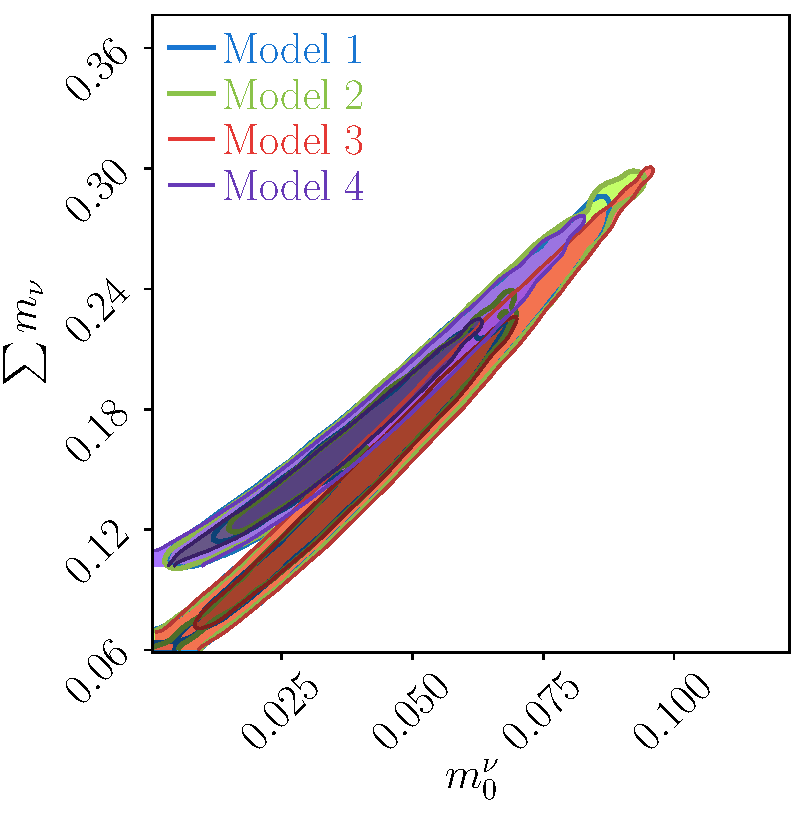
\includegraphics[scale=0.65]{Neutrino-FIGS/neutrino_hierarc_alt.pdf}
\caption[Two-dimensional (68\% and 95\% CI) marginalised posterior distributions for \NM{} and $m_0^{\nu}$ for the physically motivated models.]{Two-dimensional (68\% and 95\% CI) marginalised posterior distributions for \NM{} and $m_0^{\nu}$ for the physically motivated models, which take into account constraints from neutrino oscillation experiments. This panel shows that the current combination of cosmological data still do not have sufficient constraining power to differentiate between the two possible neutrino mass orders (or hierarchies).}
\label{fig:SumM0}
\end{center}
\end{figure}

 Nine different models were implemented to assess the impact of prior models on the upper bound of \NM{}. All models sample the basic $\Lambda$CDM parameters: $\{\Omega_b, \Omega_{cdm}, \ln 10^{10}A_s,$ $ n_s, h, \tau_{\text{reio}}\}$ as well as $N_{ur}$ to account for extra effective ultra-relativistic species. The posterior distribution analysis also contains several nuisance parameters for each of the datasets; these account for linear galaxy bias, $b(z)$, and redshift dispersion, $\sigma_s(z)$, for each of the 13 redshift tomographic bins in the BOSS dataset, two extra shot-noise parameters, $\mathcal{N}_{11}$ and  $\mathcal{N}_{12}$, for the last two bins in the BOSS dataset due to the lower number of galaxies in each of them, the absolute SNe Ia magnitude in the B-band for the Pantheon sample, $M_B^{SNe}$, and the overall Planck calibration nuisance parameter, $y_{cal}^{Planck}$. These result in a total of 30 nuisance parameters, all marginalised over after the posterior is sampled. I performed the analysis using two different nested samplers: \texttt{Multinest} \citep{2009Multinest} and \texttt{Pliny} \citep{PlinyRichardThesis}. The presented results are those from \texttt{Pliny}; the other sampler produced results that were essentially identical. %Priors for the basic $\Lambda$CDM, neutrinos, and nuisance parameters for this study are shown in Table \ref{Tb:PriorsNeutrinos}.
 
 
\qquad I performed a full cosmological analysis for all models using a combination of BOSS LSS $C_{\ell}$s, Planck CMB temperature and polarisation, Planck lensing, Type Ia SuperNovae from Pantheon, and BBN measurements of D/H data. The combination of datasets was performed at the likelihood level as described in Chapter \ref{Chap:BOSS-Cosmo}, Section \ref{Sec:CosmoAnal}. Figure \ref{fig:SumM0} shows the 2D marginalised constraints on \NM{} and $m_0^{\nu}$ for the exact models (Models 1-4). The marginalised one-dimensional posteriors for \NM{}, $N_{\text{eff}}$, and the lightest neutrino mass, $m_{0}^{\nu}$, for Models 1-7 can be found in Figure \ref{fig:neutrinoCompare1}, while the upper bounds can be found in Table \ref{Tb:Models}. The standard $\Lambda$CDM parameters, together with $N_{\text{eff}}$, are shown in Figure \ref{fig:LCDM} with the 1-$\sigma$ marginalised constraints summarised in Table \ref{tab:model_paramsLCDM}. An analysis of these results shows that all models essentially agree with each other in the $\Lambda$CDM and $N_{\text{eff}}$ parameters. Only a very small ($< 0.5 \sigma$) difference appears for the model with no massive neutrinos, Model 8, as shown in Figure \ref{fig:LCDM}.

\begin{table*}
  \centering
  \caption{Neutrino mass constraints for all models considered in this work with the 95\% CI upper bounds on both \NM, $m_{0}^{\nu}$, and $N_{\text{eff}}$. Results were obtained using a combination of BOSS $C_{\ell}$s, Planck CMB and lensing, SNe Ia from Pantheon, and BBN constraints. Models 1-4 also include constraints from oscillation experiments.}
  \label{Tb:Models}
  \begin{tabular}{c|ccc}
    \hline
    \hline
    Model & $\sum m_{\nu}$ & $m_0^{\nu}$ & $N_{\text{eff}}$\\
    & \small{[95\% CI]} & \small{[95\% CI]} & \small{[95\% CI]}\\[0.1cm]
    \hline
    \hline

     1 &  $< 0.264$ eV & $< 0.081$ eV & $3.18^{+0.38}_{-0.37}$\\
     2 & $<0.275$ eV & $< 0.086$ eV & $3.17^{+0.35}_{-0.33}$ \\
     3 &  $< 0.261$ eV & $< 0.085$ eV & $3.17^{+0.35}_{-0.33}$ \\
     4 &  $< 0.256$ & $< 0.078$ eV & $3.18\pm 0.34$ \\
     \hline
     5 & $< 0.154$ eV & -- & $3.15^{+0.35}_{-0.36}$ \\
     6 & $< 0.215$ eV & -- &  $3.16\pm 0.35$ \\
     7 & $< 0.270$ eV & -- & $3.17^{+0.38}_{-0.35}$ \\
     \hline
     8 & -- & -- & $3.14\pm 0.35$ \\
     9 & -- & -- & $3.14^{+0.35}_{-0.33}$ \\
     \hline
     \hline
  \end{tabular}
\end{table*}

%\RED{Should I check and mention something about nuisance params?}
\begin{figure}
\begin{center}
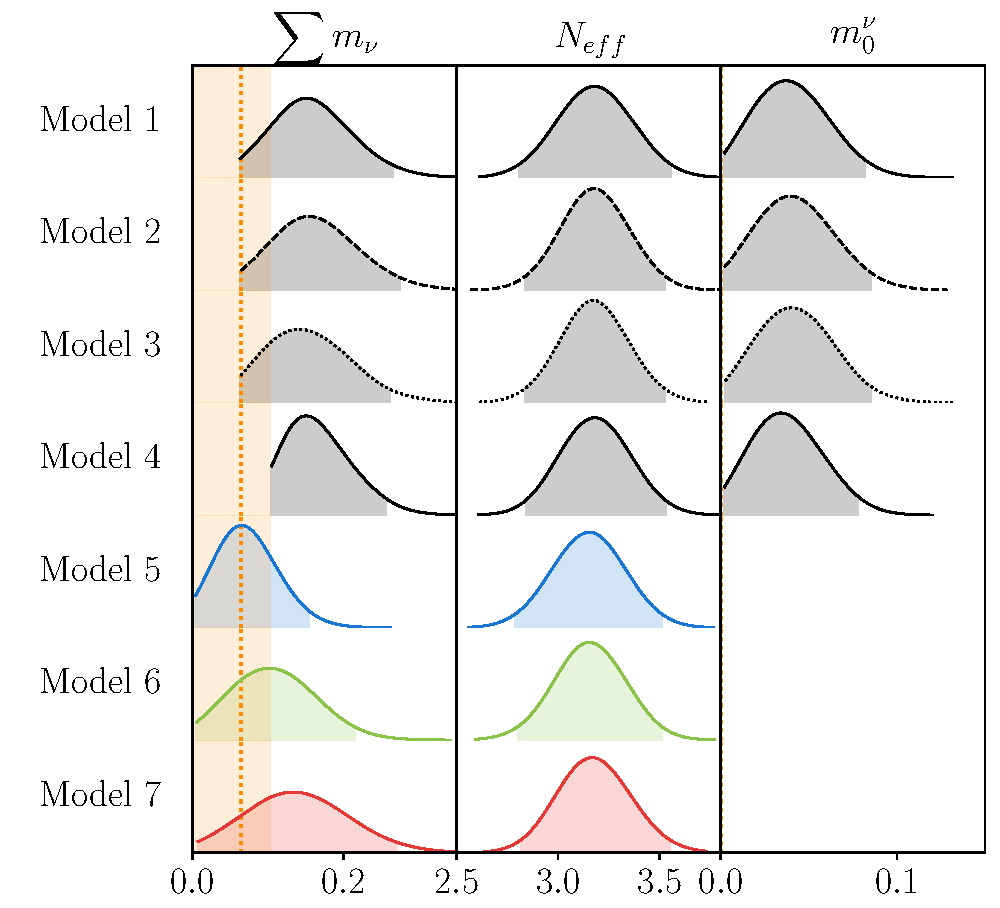
\includegraphics[width=\columnwidth]{Neutrino-FIGS/neutrino_prior_models.pdf}
\caption[Results for neutrino related parameters from the neutrino model prior analysis.]{The marginalised posterior probabilities for neutrino-related parameters for a range of neutrino models with 95\% CI shaded regions for neutrino parameters. Exact models (Models 1-4) yield  robust constraints for the upper bound of $\sum m_{\nu} \lesssim 0.26$ eV (95\% CI) and for the lightest neutrino mass $m_0^{\nu} \lesssim 0.086$ eV (95\% CI), while models with cosmological approximations (Models 5-7) have up to 43\% variation for the upper bound of $\sum m_{\nu}$ at 2-$\sigma$ CI. The vertical dashed line in the left plot shows the minimum possible value for $\sum m_{\nu}$ for the NH while the shaded region shows the same for the IH. All models also sample the $\Lambda$CDM parameters, shown in Figure \ref{fig:LCDM}. All results shown  were obtained by varying $N_{\text{eff}}$ and therefore present a wider, stronger statement than would have been the case for a fixed value of $N_{\text{eff}}$. }
\label{fig:neutrinoCompare1}
\end{center}
\vspace{-2.5mm}
\end{figure}
\qquad The marginalised posteriors for \NM{} (Figure \ref{fig:neutrinoCompare1}) show that the use of exact models yield robust upper bounds at 95\% CI, varying between $< 0.256$ eV and $<0.275$ eV. The models in which the hierarchy was also sampled, Models 1 and 2, did not demonstrate a significant choice between NH and IH; therefore, I marginalised over the hierarchy to get the results shown in Figure \ref{fig:neutrinoCompare1}. Meanwhile, the commonly used cosmological approximations demonstrate a variation in the 95\% CI upper bound of 43\% between Models 5 and 7: $\sum m_{\nu} < 0.154$ eV and $\sum m_{\nu} < 0.270$ eV, respectively. This indicates that such approximations can be problematic and that the upper bounds obtained are dominated by the prior model choice.

\qquad The nested sampler used in the cosmological analysis provides us with Bayesian evidences for each of the models. The ratio of evidences between two models, known as the Bayes factor, quantifies statistically if either is more strongly supported by the data \citep{1995BayesFactor}. The Bayes factors for all other pairs of models were consistent with one to within the statistical precision of the nested sampling algorithm, meaning that the data considered in this work do not strongly support any one of our models over the others.

\section{Conclusions}
\begin{figure}
\begin{center}
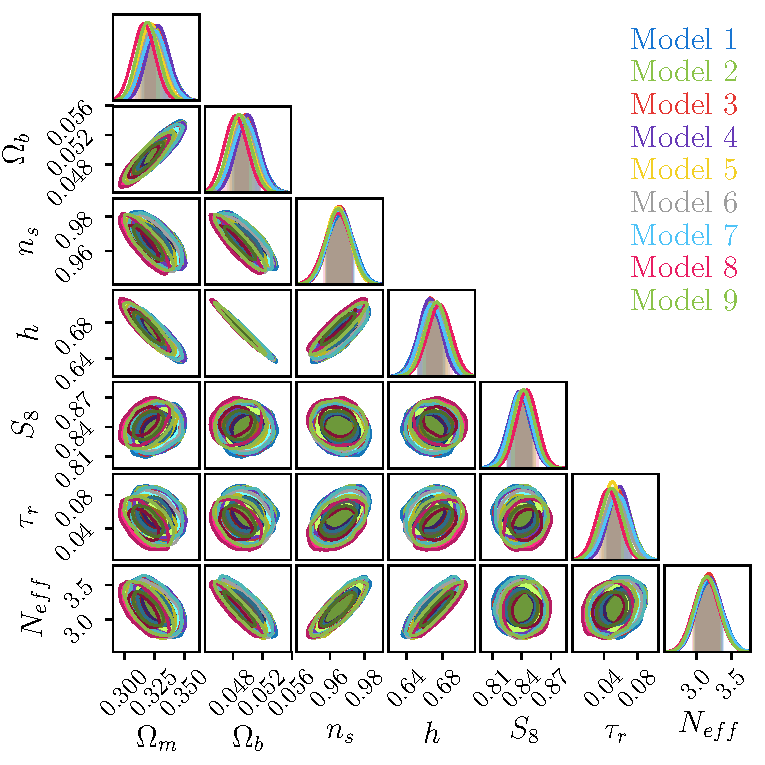
\includegraphics[width=\columnwidth]{Neutrino-FIGS/LCDM_Params_prl_alt.pdf}
\caption[One- (68\% CI) and two-dimensional (68\% and 95\% CI) marginalised posterior distributions for the relevant sampled and derived $\Lambda$CDM parameters in each of the nine different models.]{One- (68\% CI) and two-dimensional (68\% and 95\% CI) marginalised posterior distributions for the relevant sampled and derived $\Lambda$CDM parameters considered in each of the nine different models (where, $S_8 \equiv \sigma_8\sqrt{\Omega_m/0.3})$. All models agree in the basic $\Lambda$CDM parameters and for $N_{\text{eff}}$ to within half-$\sigma$ or less; Model 8 is an outlier among the models, since it contains no massive neutrinos, and hence often yields a mild outlier among the marginalised posterior distributions. This results address the issue of how the modelling of neutrinos should be done within a standard $\Lambda$CDM analysis where the \NM{} is not the main focus of the analysis. It is clear that the simpler approach, leading to no biases, is the one taken by Model 9 (same as in \cite{PlanckCosmology2016,2018PlanckCosmology}).  Finally, note that changing the neutrino mass modelling does not affect $N_{\text{eff}}$. This suggests that if one wishes to study $N_{\text{eff}}$, the particular model chosen for the neutrino masses does not seem to play a role.}
\label{fig:LCDM}
\end{center}
\end{figure}


In this chapter I have shown that the choice of how the neutrino is modelled for cosmological purposes significantly affects current upper bounds for the sum of the neutrino masses. If physically motivated exact models are chosen, the upper bound is found to be $\sum m_{\nu} < 0.264$ eV (95\% CI). On the other hand, we now possess enough cosmological data to show that this upper bound is significantly different if one makes the approximation that one (two) of the neutrino mass eigenstates have zero mass and that the mass is contained in the other two (one) eigenstates. 

\qquad Here, I show a concise framework, applied to the largest spectroscopic galaxy survey to date, to obtain robust neutrino mass information from a combination of cosmological observations and particle physics constraints. Even though no model was preferred from a Bayesian evidence analysis, cosmological approximations can cause a variation up to 44\% on the upper bound of \NM{}, while all exact models yield results that vary only by 7\% for the upper bound (both considered at 95\% CI). Using this exact modelling methodology, I present what it is believed to be one of the first cosmological measurement of the upper bound of the lightest neutrino mass species: $m_{0}^{\nu} < 0.086$ eV at 95\% CI. Even though the posterior distributions for $m_{0}^{\nu}$ in Figure \ref{fig:neutrinoCompare1} exhibits a peak, I do not claim it to be a detection as Bayes factor analysis between models were inconclusive and zero is still within the 95\% CI.

\qquad In light of these results, I argue that the approach presented here as Model 1 should be the choice for current and future cosmological neutrino mass investigations (given the volume of data now available to cosmologists). One should no longer make approximations assuming a degenerate neutrino mass spectrum as this could lead to potentially nonphysical upper bounds and constraints. Instead, one should make use of a cosmological analysis that takes into account both of the neutrino mass hierarchies, as well as particle physics constraints and their uncertainties. 

\qquad Finally, I demonstrated here that, if neutrino masses are not the interest of the analysis, the simplest model which fixes the sum of neutrino masses to the particle physics lower bound for the NH, $\sum m_{\nu} = 0.06$ eV, yields reliable cosmological results in the $\Lambda$CDM model context. In other words, a standard $\Lambda$CDM analysis is independent of the fiducial choice for the neutrino mass model, allowing for a simple approach to be taken. I emphasise that one should consider massive neutrinos for a standard $\Lambda$CDM analysis -- as the data is sensitive enough, as seen in the difference between the model with zero massive neutrinos (Model 8) and all others in Figure \ref{fig:LCDM}. The exact approach for neutrino mass estimation will be extremely relevant for future cosmological neutrino studies in the analysis of the next generation of surveys, e. g. DESI \citep{2016-DESI}, Euclid \citep{2011EuclidRedPaper}, LSST \citep{LSST}, and J-PAS \citep{JPAS}.


\begin{landscape}
\begin{table}
    \centering
    \caption[Marginalised $\Lambda$CDM parameters constraints and 68\% credible intervals for all 9 models considered.]{Marginalised $\Lambda$CDM parameters constraints and 68\% credible intervals for all 9 models considered. All constraints were obtained from a combination of BOSS LSS $C_{\ell}$s, Planck CMB temperature and polarisation, Planck lensing, Type Ia SuperNovae from Pantheon, and BBN measurements of D/H data}
    \label{tab:model_paramsLCDM}
    {\begin{tabular}{c|ccccccc}
        \hline
        \hline
		Model & $\Omega_m$ & $\Omega_b$ & $n_s$ & $h$ & $S_8$ & $\tau_{r}$ & $N_{\text{eff}}$\\ 
		\hline
		\hline
	1 & $0.327\pm 0.011$ & $\left( 49.8^{+1.8}_{-1.7} \right) \times 10^{-3}$ & $\left( 966.1^{+7.5}_{-7.7} \right) \times 10^{-3}$ & $0.667\pm 0.014$ & $0.837^{+0.011}_{-0.012}$ & $0.058\pm 0.014$ & $3.18\pm 0.19$ \\ 
		2 & $\left( 327.3^{+9.8}_{-9.6} \right) \times 10^{-3}$ & $\left( 50.0\pm 1.6 \right) \times 10^{-3}$ & $\left( 965.7^{+7.2}_{-6.8} \right) \times 10^{-3}$ & $0.666\pm 0.013$ & $0.837\pm 0.011$ & $0.059^{+0.013}_{-0.014}$ & $3.17^{+0.18}_{-0.17}$ \\ 
		3 & $\left( 326.9^{+9.1}_{-9.2} \right) \times 10^{-3}$ & $\left( 49.9^{+1.5}_{-1.6} \right) \times 10^{-3}$ & $\left( 965.4^{+7.1}_{-6.5} \right) \times 10^{-3}$ & $0.667\pm 0.012$ & $0.838^{+0.012}_{-0.011}$ & $0.058\pm 0.014$ & $3.17^{+0.18}_{-0.17}$ \\ 
		4 & $\left( 328.0^{+9.2}_{-9.5} \right) \times 10^{-3}$ & $\left( 50.0^{+1.6}_{-1.5} \right) \times 10^{-3}$ & $\left( 965.7^{+7.2}_{-7.0} \right) \times 10^{-3}$ & $0.666^{+0.013}_{-0.012}$ & $0.838\pm 0.011$ & $0.058\pm 0.013$ & $3.18^{+0.17}_{-0.18}$ \\ 
		5 & $\left( 321.8^{+9.3}_{-9.0} \right) \times 10^{-3}$ & $\left( 49.1^{+1.6}_{-1.5} \right) \times 10^{-3}$ & $\left( 964.5\pm 6.8 \right) \times 10^{-3}$ & $0.671\pm 0.013$ & $0.842\pm 0.011$ & $0.050\pm 0.012$ & $3.15\pm 0.18$ \\ 
		6 & $\left( 323.3^{+10.3}_{-9.3} \right) \times 10^{-3}$ & $\left( 49.4^{+1.7}_{-1.5} \right) \times 10^{-3}$ & $\left( 965.2^{+7.0}_{-7.3} \right) \times 10^{-3}$ & $0.670\pm 0.013$ & $0.840\pm 0.011$ & $0.053\pm 0.014$ & $3.16^{+0.18}_{-0.17}$ \\ 
		7 & $0.325\pm 0.010$ & $\left( 49.7\pm 1.7 \right) \times 10^{-3}$ & $\left( 965.6^{+7.3}_{-7.2} \right) \times 10^{-3}$ & $0.668^{+0.014}_{-0.013}$ & $0.838^{+0.012}_{-0.011}$ & $0.057^{+0.014}_{-0.015}$ & $3.17^{+0.19}_{-0.18}$ \\ 
		8 & $\left( 316.2^{+9.2}_{-9.1} \right) \times 10^{-3}$ & $\left( 48.3^{+1.6}_{-1.5} \right) \times 10^{-3}$ & $\left( 964.6^{+7.4}_{-7.7} \right) \times 10^{-3}$ & $0.677\pm 0.013$ & $0.845\pm 0.011$ & $0.045^{+0.013}_{-0.014}$ & $3.14\pm 0.18$ \\ 
		9 & $\left( 319.3^{+9.2}_{-8.7} \right) \times 10^{-3}$ & $\left( 48.9^{+1.6}_{-1.5} \right) \times 10^{-3}$ & $\left( 964.7\pm 7.1 \right) \times 10^{-3}$ & $0.673\pm 0.013$ & $0.842\pm 0.011$ & $0.049\pm 0.013$ & $3.14^{+0.18}_{-0.17}$ \\ 
		\hline
		\hline
    \end{tabular}}
\end{table}
\end{landscape}
